
% justificar en 4 renglones o menos porque usamos x patron de arquitectura
% identificar cuales son los requerimientos no funcionales
% hacer la matriz donde aparecen las vistas y los requerimientos por el otro lado
% marcar en cada celda el impacto que tiene cada uno en las vistas (suma puntos justificar cada marcada)
% ej es importante la performance - x en performance y las vistas impactados - afecta en concurrencia por tal cosa
% si tenemos dudas de algo, suponemos sobre eso.
% foto del documento y/o libreta - incluir en el archivo
% a las 9 se inhabilita el espacio de entrega
% a las 7 se habilita
% son 2 horas
% minutos antes subir respuesta

\section{Presentación de una arquitectura}
La arquitectura de software es aquellas decisiones que son importantes y difíciles de cambiar.
Para armar un informe donde queremos transmitir alguna información debemos tener presente que es lo que queremos contar y a quien.
Un documento de arquitectura esta dirigido a muchos interesados, desarrolladores, lideres de proyecto, algún usuario, encargados de infraestructura, despliegue, bases de datos.

\subsubsection*{¿Como hacemos para escribir un único documento para todos ellos?}
Usamos el modelo de Vistas 4+1 que permite a cada interesado encontrar lo que necesitan saber acerca de la arquitectura.

\begin{figure}[!htb]
    \centering
    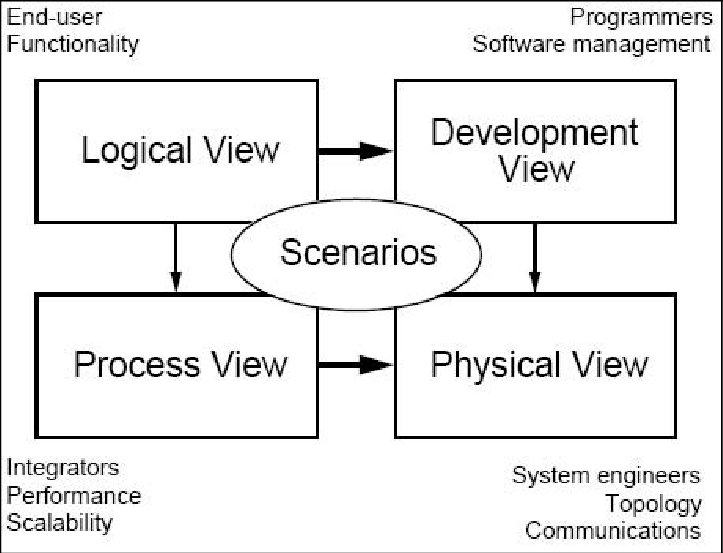
\includegraphics[width=0.6\textwidth]{img/4+1.png}
\end{figure}

\textit{Se puede leer el paper }\href{https://www.cs.ubc.ca/~gregor/teaching/papers/4+1view-architecture.pdf}{aquí}

\subsection*{Vista lógica}
\begin{itemize}
\item Tratar de poner los requisitos funcionales (los relevantes). Se aplican los principios de encapsulamiento y herencia.
\item Diagramas de estados, clases, secuencia y actividad son herramientas que vamos a necesitar en esta vista.
\item Le interesa al usuario final.
\end{itemize}


\subsection*{Vista de desarrollo (o componentes)}
\begin{itemize}
\item Se centra en la organización de los módulos de software en el ambiente de desarrollo del software.
\item Tiene en cuenta los requisitos internos relativos a la facilidad de desarrollo, administración del software, reutilización y elementos comunes, y restricciones impuestas por las herramientas.
\item Usamos diagramas de componentes.
\item Le interesa al desarrollador.
\end{itemize}



\subsection*{Vista procesos}
\begin{itemize}
\item Se centra en requisitos no funcionales tales como rendimiento, disponibilidad, tolerancia ante fallas e integridad.
\item Relacionada con la de componentes.
\item Se usan diagramas de clases
\item Le interesa al diseñador del sistema y al que lo integre.
\end{itemize}


\subsection*{Vista física (o despliegue)}
\begin{itemize}
\item Toma en cuenta los requisitos no funcionales de escalabilidad, performance y disponibilidad.
\item Le interesa al diseñador del sistema.
\end{itemize}


\subsection*{Vista de Escenarios}
\begin{itemize}
\item Para que escenarios estamos planteando nuestra solución. Son una abstracción de los requisitos mas importantes.
\item Le interesa al usuario final.
\item Busca ver el entendimiento del sistema.
\end{itemize}

